%
% -- Manlio Modugno

\documentclass{beamer} 
\usepackage{eulervm}
%\usepackage{booktabs}
\usepackage{listings}
\usepackage{bold-extra}
\usepackage{cancel}
\usepackage{fancybox}
\usepackage{soul}
\usepackage[english]{babel}
\usepackage[utf8]{inputenc}
\usepackage{hyperref}
\usepackage{amsmath}
%\hypersetup{colorlinks=true,urlcolor=blue}

\newcommand{\codefont}{\fontsize{6}{8}\selectfont}
\lstset{language=[Sharp]C, 
captionpos=b, 
frame=lines,
lineskip= 1pt, %space between lines
basicstyle=\codefont, 
keywordstyle=\color{blue}, 
commentstyle=\color{green}, 
stringstyle=\color{red}, 
numbers=left, 
numberstyle=\tiny, 
stepnumber=2,
numbersep=5pt,
breaklines=true, 
breakatwhitespace=false,
showstringspaces=false,
frame=single,
tabsize=2,
emph={double,bool,int,unsigned,char,true,false,void},
emphstyle=\color{blue},
emph={Assert,Test},
emphstyle=\color{red},
emph={[2]\using,\#define,\#ifdef,\#endif},
emphstyle={[2]\color{blue}}
}


\mode<presentation>
\definecolor{title_color}{RGB}{2,128,181} 
\usetheme{Ilmenau}
\usecolortheme[named=title_color]{structure}
\setbeamercolor{palette quaternary}{use=structure,fg=black,bg=white} %header footer color
\useoutertheme[subsection=false]{smoothbars}
\setbeamercovered{transparent}
\setbeamertemplate{navigation symbols}{}
\setbeamerfont{subsection in toc}{size=\scriptsize}

\title{The Liskov Substitution Principle}
\author{Manlio Modugno}
\institute[GMTechnologies] 

\date[]{The Liskov Substitution Principle}

\subject{}

\graphicspath{{img/}}
\pgfdeclareimage[height=0.6cm]{mfg-logo}{img/mfgLogo}
\logo{\pgfuseimage{mfg-logo}}

%
% Content start
%
\begin{document}
\begin{frame}
  \titlepage
\end{frame}

\begin{frame}
  \frametitle{Topics}
  \tableofcontents
\end{frame}


\section{Intro}
\subsection{Intro}
\begin{frame}
  \frametitle{Intro}
  \begin{itemize}
	\item<+-> OCP based (usually) on abstraction and polymorphism..
	\item<+-> In statically typed languages, abstraction and polymorphism, are supported by inheritance.
	\item<+-> How to take care of inheritance when applying OCP ..? 
    \item<+-> using LSP def:\textbf{Subtypes must be substitutable for their base types.}
   \end{itemize}
\end{frame}

\subsection{Consequences}
\begin{frame}[containsverbatim]
	\frametitle{Consequences}
	Consider f taking B. Here we say that D is violating LSP \\
	A LSP violation $ \rightarrow $ an OCP violation, because usually some special action is taken to handle 'special' case.. \\
	\begin{lstlisting}
	interface B { void do() };
	class D implements B { 
		public void do(){
			throw new RunTimeException("boom!")
		}
	}
	....
	f(B ref){
		if(!(ref instanceof D)){  //OCP violation
			ref.do();	
		}
	}	
	...
	\end{lstlisting}
\end{frame}

\section{Example}
\subsection{Example: simple violation}
\begin{frame}[containsverbatim]
	\frametitle{Example: simple violation}
	\textit{DrawShape} violates OCP, it must knows every possible derivative of \textit{Shape} .. \\
	\begin{lstlisting}
struct Point {double x, y;}
public enum ShapeType {square, circle};
public class Shape{
	private ShapeType type;
	public Shape(ShapeType t){type = t;}
	public static void DrawShape(Shape s){
		if(s.type == ShapeType.square)
			(s as Square).Draw();
		else if(s.type == ShapeType.circle)
			(s as Circle).Draw();
	}
}
public class Circle : Shape { void Draw() {...} }
public class Square : Shape { void Draw() {...} }

	\end{lstlisting}
	\textit{Square} and \textit{Circle} cannot be substituted using \textit{Shape} (no abstract polymorphic method draw). This is a LSP violation, that in turns forces an OCP one.  \\
\end{frame}


\subsection{Example: subtle violation}
\begin{frame}[containsverbatim]
	\frametitle{Example: subtle violation}
	Starting from an existing class a new requirement comes..(i.e. ``we'd like to maage Squares) \\
	\begin{lstlisting}
public class Rectangle{
	private Point topLeft;
	private double width;
	private double height;
	public double Width{
		get { return width; }
		set { width = value; }
	}
	public double Height{
		get { return height; }
		set { height = value; }
	}
}
	\end{lstlisting}
\end{frame}

\begin{frame}
  \frametitle{IS-A relationship}
  \begin{itemize}
	\item<+-> Pay attention to IS-A mantra ``if a new kind of object can fulfill the IS-A relationship with an old kind of object, the class of the new object should be derived from the class of the old object''
	\item<+-> For all normal (i.e. natural) purposes a square is a rectangle.. but this is a too weak! definition!
   \end{itemize}
\end{frame}

\begin{frame}
  \frametitle{IS-A relationship: Rectangle vs Square}
  \begin{itemize}
	\item<+-> A first clue that something is weird is that \textit{Square} doesn't need both height and width..
	\item<+-> Depending on our context, using both variables can be a problem or not..
	\item<+-> A real design problem here is the inherit of setter properties.. a \textit{Square} doesn't need them since height and width are identical..
   \end{itemize}
\end{frame}

\begin{frame}[containsverbatim]
	\frametitle{IS-A relationship: Rectangle vs Square, no problem ! I've got a solution!}
	I can override properties to fix things... and mathematically \textit{Square} is correct\\
	\begin{lstlisting}
class Square {
public new double Height{ set {
    base.Height = value;
    base.Width = value;
  }
 }
 public new double Height{ set {
    base.Height = value;
    base.Width = value;
  }
 }
}
...
Square s = new Square();
s.SetWidth(1); // Fortunately sets the height to 1 too.
s.SetHeight(2); // sets width and height to 2. Good thing.

	\end{lstlisting}
\end{frame}

\begin{frame}[containsverbatim]
	\frametitle{LSP violation}
	But if in the code already exists a function like: \\
	\begin{lstlisting}
void g(Rectangle r){
  r.Width = 5;
  r.Height = 4;
  if(r.Area() != 20)
    throw new Exception("Bad area!");
}
	\end{lstlisting}
	we have a problem... \\
\end{frame}

\begin{frame}
  \frametitle{LSP violation of g function}
  \begin{itemize}
	\item<+-> Author of g assumed that changing the width of a Rectangle leaves its height unchanged (and this is reasonable!)
	\item<+-> g is fragile with respect to Square / Rectangle hierarchy.. because a \textit{Square} \textbf{it's not} a \textit{Rectangle}! (in this context)
	\item<+-> One might argue that developer of g function had no right to make assumption of independent measure between height and width...
	\item<+-> but here, real error is the hierarchy created by second developer that broke an invariant of \textit{Rectangle} inserting a \textit{Square}!
   \end{itemize}
\end{frame}

\subsection{Validity is not intrinsic}
\begin{frame}
  \frametitle{Validity is not intrinsic}
  \begin{itemize}
	\item<+-> LSP leads to an important conclusion: ``A model, viewed in isolation, cannot be meaningfully validated''
	\item<+-> ..the validity of a model can be expressed only in terms of
its clients.. in fact \textit{Rectangle} and \textit{Square} taken in isolation were valid..
	\item<+-> ..but when used from a client model broke down...
	\item<+-> When considering whether a particular design is appropriate, one cannot simply view the solution in isolation.
	\item<+-> \textbf{One must view it in terms of the reasonable assumptions made by the users of that
design} (...pay attention to needless complexity!)
   \end{itemize}
\end{frame}

\subsection{ISA is about behavior}
\begin{frame}
  \frametitle{ISA is about behavior}
  \begin{itemize}
	\item<+-> Why something went wrong with Rectangle/Square relationship..? 
	\item<+-> isn't a Square a Rectangle ..? Isn't so natural..?
	\item<+-> maybe for everyone except that for g's author...
	\item<+-> \textbf{Behavior} of \textit{Square} is not consistent with g's expectation.. 
	\item<+-> \textbf{Behaviorally a Square is not a Rectangle!}.. and it is behavior that software is really all about
	\item<+-> LSP make a strict definition for subtype relationship
   \end{itemize}
\end{frame}

\subsection{Design by contract}
\begin{frame}
  \frametitle{Design by contract}
  \begin{itemize}
	\item<+-> How to know what clients behaviorally expect?
	\item<+-> Using DBC, the author of a class explicitly states the contract for that class.
	\item<+-> ..could be tricky.. writing test It's better..
   \end{itemize}
\end{frame}

\section{A Real-World Example}
\subsection{Motivation}
\begin{frame}
  \frametitle{A Real-World Example}
  \begin{itemize}
	\item<+-> Author purchased a third-party lib that managed \textit{Bag}s and \textit{Set}s data structure..
	\item<+-> Exist two variety \textit{bounded}, based on array, and \textit{unbounded}, based on linked list
	\item<+-> \textit{BoundedSet} specify by constructor max size of elements...
	\item<+-> \textit{UnoundedSet} has not limit in size allocation..
	\item<+-> To avoid coupling author wrapped libraries in his own interfaces
   \end{itemize}
\end{frame}

\subsection{wrapping}
\begin{frame}
  \frametitle{A Real-World Example}
  \fbox{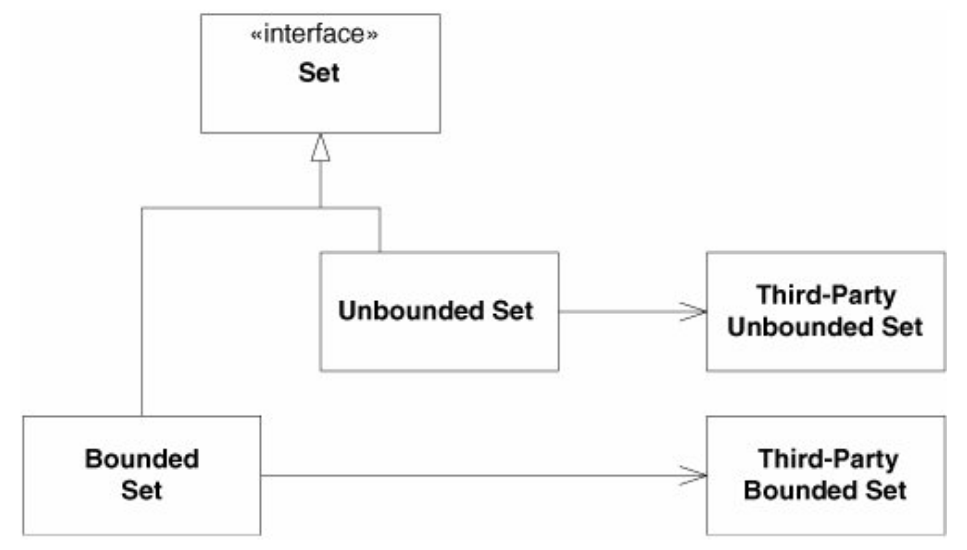
\includegraphics[scale=0.3]{wrap}}
\end{frame}

\begin{frame}[containsverbatim]
	\frametitle{A Real-World Example}
	Interface \textit{Set} to unify unbounded and bounded variety\\
	\begin{lstlisting}
	public interface Set{
      void Add(object o);
      void Delete(object o);
      bool IsMember(object o);
	}
    ...
    void PrintSet(Set s){
	  foreach(object o in s)
  	  Console.WriteLine(o.ToString());
	}	
	\end{lstlisting}
\end{frame}

\begin{frame}
  \frametitle{A Real-World Example}
  \begin{itemize}
	\item<+-> It's nice to don't care about what kind of Set to use... 
	\item<+-> It's up to programmer to choose which kind to use.. for memory / speed issues..
	\item<+-> ...
   \end{itemize}
\end{frame}

\subsection{problem}
\begin{frame}
  \frametitle{Problem}
	Author added a \textit{PersistentSet} that can be stored and retrieved..The third-party version defined accept only \textit{PersistentObject} \\
	\begin{center}
	\fbox{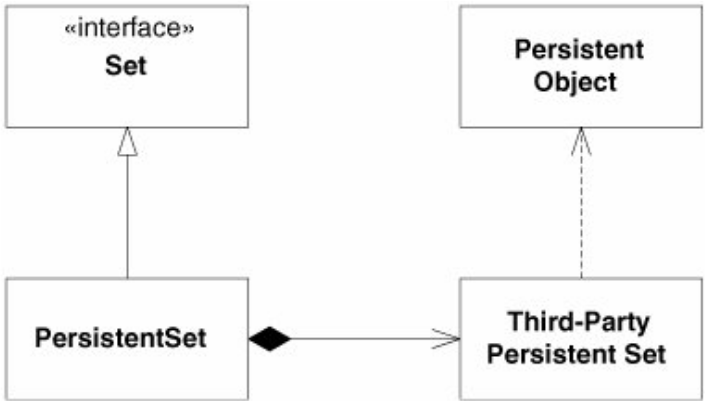
\includegraphics[scale=0.3]{persistent}}
	\end{center}
\end{frame}

\begin{frame}[containsverbatim]
  \frametitle{Problem}
  \begin{itemize}
	\item When a client is adding members to the base class Set, that client cannot be sure whether the Set might be a PersistentSet 
	\item ... so It can't know whether the elements it adds should be derived from \textit{PersistentObject}
	\item code like PersistentSet\#Add introduce potential runtime problems..
	\item Existing functions that used \textit{Set} as reference in signature can now broke down because of \textit{PersistentSet}
   \end{itemize}
   \begin{lstlisting}
//PersistentSet#Add
   
void Add(object o){
  PersistentObject p = (PersistentObject)o;
  thirdPartyPersistentSet.Add(p);
}
	\end{lstlisting}
\end{frame}

\subsection{First solution, not conforming to LSP}
\begin{frame}
  \frametitle{First solution, not conforming to LSP}
	\begin{itemize}
	\item<+-> A first approach was by convention..   
	\item<+-> ...it's a powerful principle.. but can have drawbacks..
	\item<+-> an unfocused developer can violate conventions...
	\item<+-> ...we should share conventions and than change them if necessary..
   \end{itemize}
\end{frame}

\subsection{An LSP-compliant solution}
\begin{frame}
  \frametitle{An LSP-compliant solution}
	\begin{itemize}
	\item<+-> \textit{PersistentSet} is not a subtype of \textit{Set} yet they share some feature...
	\item<+-> ...it's only the \textit{add} method that cause problem with LSP
   \end{itemize}
\end{frame}

\begin{frame}
  \frametitle{An LSP-compliant solution}
	A new interface is defined with common features \\
	\begin{center}
	\fbox{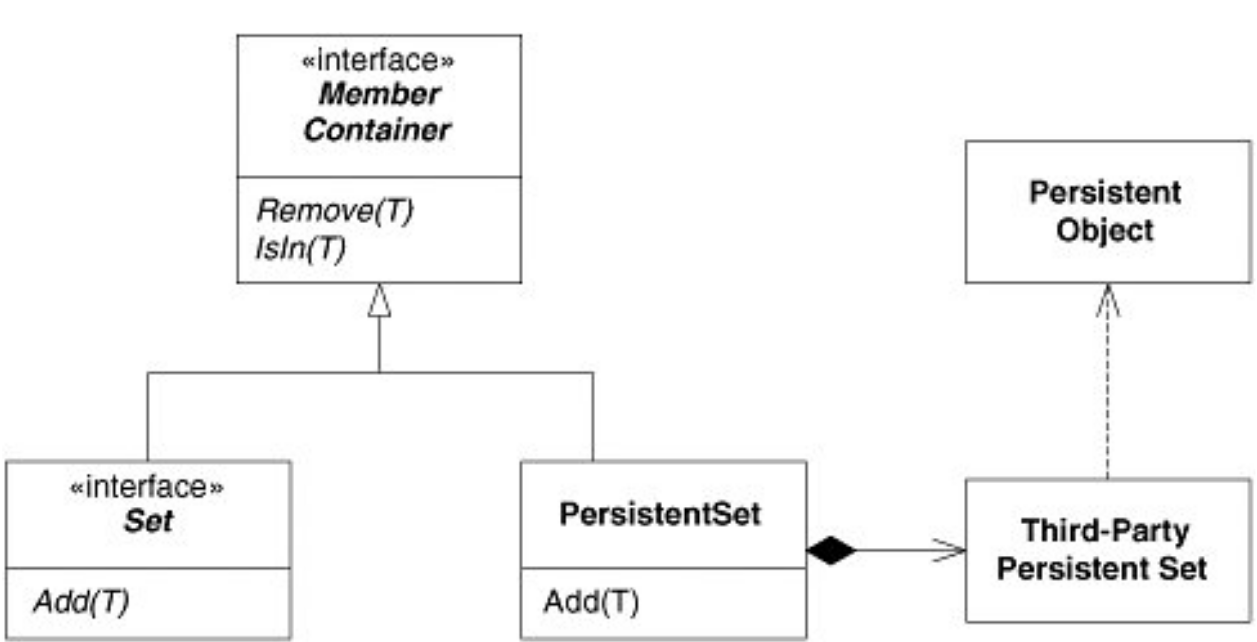
\includegraphics[scale=0.22]{lspGood}}
	\end{center}
\end{frame}

\section{Factoring Instead of Deriving}
\subsection{Factoring Instead of Deriving}
\begin{frame}[containsverbatim]
	\frametitle{Factoring Instead of Deriving}
	At first, these two classes appear to be \textbf{natural} candidates for inheritance. \textit{LineSegment} needs every member variable and every member function declared in \textit{Line} and override \textit{isOn}\\
	\begin{lstlisting}
public class Line{
  private Point p1;
  private Point p2;
  public Line(Point p1, Point p2){this.p1=p1; this.p2=p2;}
  public Point P1 { get { return p1; } }
  public Point P2 { get { return p2; } }
  public double Slope { get {/*code*/} }
  public double YIntercept { get {/*code*/} }
  public virtual bool IsOn(Point p) {/*code*/}
}
public class LineSegment : Line{
  public LineSegment(Point p1, Point p2) : base(p1, p2) {}
  public double Length() { get {/*code*/} }
  public override bool IsOn(Point p) {/*code*/}
}
	\end{lstlisting}
\end{frame}

\begin{frame}
  \frametitle{Factoring Instead of Deriving}
	\begin{itemize}
	\item<+-> A user of \textit{Line} in a plane (as function!) has the right to expect that isOn(YIntercept) is always true...
	\item<+-> .. but for a \textit{Segment} this is not always true!
	\item<+-> depending on context, a compromise can be \textbf{profitable} than perfection.. 
	\item<+-> However, conformance to LSP should not be surrendered lightly..
   \end{itemize}
\end{frame}

\begin{frame}[containsverbatim]
	\frametitle{Factoring Instead of Deriving}
	\textit{LinearObject}factors out the common functionalities excluding \textit{IsOn} method. Users of \textit{Line} are safe and assumption od \textit{isOn} cannot be made\\
	\begin{lstlisting}
public abstract class LinearObject{
  private Point p1;
  private Point p2;
  public LinearObject(Point p1, Point p2)  {this.p1=p1; this.p2=p2;}
  public Point P1 { get { return p1; } }
  public Point P2 { get { return p2; } }
  public double Slope { get {/*code*/} }
  public double YIntercept { get {/*code*/} }
  public virtual bool IsOn(Point p) {/*code*/}
}
public class Line : LinearObject{
  public Line(Point p1, Point p2) : base(p1, p2) {}
  public override bool IsOn(Point p) {/*code*/}
}
public class LineSegment : LinearObject{
  public LineSegment(Point p1, Point p2) : base(p1, p2) {}
  public double GetLength() {/*code*/}
  public override bool IsOn(Point p) {/*code*/}
}
	\end{lstlisting}
\end{frame}


\section{Heuristics and Conventions}
\subsection{Heuristics and Conventions}
\begin{frame}
  \frametitle{How to smell LSP violations?}
  \begin{itemize}
	\item<+-> Derivative classes somehow remove functionality from their base classes..
	\item<+-> A derivative that does less than its base is usually not substitutable for that base and therefore violates LSP
	\item<+-> degenerate function (i.e. empty function) can be indicative of LSP violation
   \end{itemize}
\end{frame}

\section{Conclusion}
\subsection{Conclusion}
\begin{frame}
  \frametitle{Conclusion}
  \begin{itemize}
	\item<+-> OCP keep applications maintainable, reusable and robust..
	\item<+-> LSP is one of the prime enablers of OCP.. because substitutability of subtypes allows a
module, expressed in terms of a base type, to be extensible without modification
	\item<+-> The term IS-A is too broad to act as a definition of a subtype. The true definition of a subtype is substitutable, where substitutability is defined by either an explicit or implicit contract.
   \end{itemize}
\end{frame}

\end{document}
